\chapter[Computer-based Mechanisms and Procedures to Gamify CL Sessions]{Computer-based Mechanisms and Procedures to Gamify Collaborative Learning Sessions}
\label{chapter:computer-based-mechanisms-procedures}

The purpose of this chapter is to show how the ontology OntoGaCLeS, and the GIMF model, presented in previous chapters, can be used in intelligent theory-aware systems to gamify CL sessions, and thus, to deal with the motivation problem caused by the scripted collaboration.
The \autoref{sec:conceptual-flow-gamify-cl-sessions} presents a conceptual flow to gamify CL sessions proposed as a computer-based procedure that should be used by intelligent theory-aware systems to extract knowledge encoded in the ontology OntoGaCLeS, and then to provide suggestions based on theoretical justification.
In \autoref{sec:reference-architecture}, a reference architecture based on the conceptual flow to gamify CL sessions is presented.
This architecture has been proposed to support the building of computer-based mechanisms that provide support in intelligent-theory aware systems for dealing with the motivation problem caused by the scripted collaboration.

Part of the work described in this chapter was published by the author of this PhD thesis dissertation in the scientific
articles:

\begin{itemize}
\item \aspas{\emph{An Ontology Engineering Approach to Gamify Collaborative Learning Scenarios}} published in the 20\textsuperscript{th} International Conference on Collaboration and Technology, CRIWG 2014, held in Santiago, Chile \cite{ChallcoMoreiraMizoguchiIsotani2014}.

\item \aspas{\emph{Gamification of Collaborative Learning Scenarios: Structuring Persuasive Strategies Using Game Elements and Ontologies}} published in the 1\textsuperscript{st} International Workshop on Social Computing in Digital Education, SocialEdu 2015, held in Stanford, CA, USA \cite{ChallcoMizoguchiBittencourtIsotani2015}.
\end{itemize}

%%%%%%%%%%%%%%%%%%%%%%%%%%%%%%%%%%
\section[Conceptual Flow to Gamify CL Sessions Using the Ontology OntoGaCLeS]{Conceptual Flow to Gamify Collaborative Learning Sessions Using the Ontology OntoGaCLeS}
\label{sec:conceptual-flow-gamify-cl-sessions}

As was mentioned before in previous chapters, to avoid the motivation problem caused by the scripted collaboration towards the gamification, it is necessary to solve the context-dependency related to the participants, and the context-dependency related to the target behavior being gamified.
In this sense, the gamification should be applied in the most concrete level of CL scenarios in which the content-domain and participants are well defined.
This kind of CL scenario is the CL session, a scenario in which the group members, CL roles and sequencing of actions to be performed by the group members are well established.

\autoref{fig:conceptual-flow-gamify-cl-sessions} shows the conceptual flow proposed to gamify CL sessions using the ontology OntoGaCLeS.
This flow has been developed from the viewpoint of an instructional designer who employs suggestions given by intelligent-theory aware systems, which in turn use the knowledge encoded in the ontology OntoGaCLeS as a source of information to provide these suggestions.

\begin{figure}[htb]
  \caption{Conceptual flow to gamify collaborative learning sessions using the ontology OntoGaCLeS}
  \label{fig:conceptual-flow-gamify-cl-sessions}
  \centering
  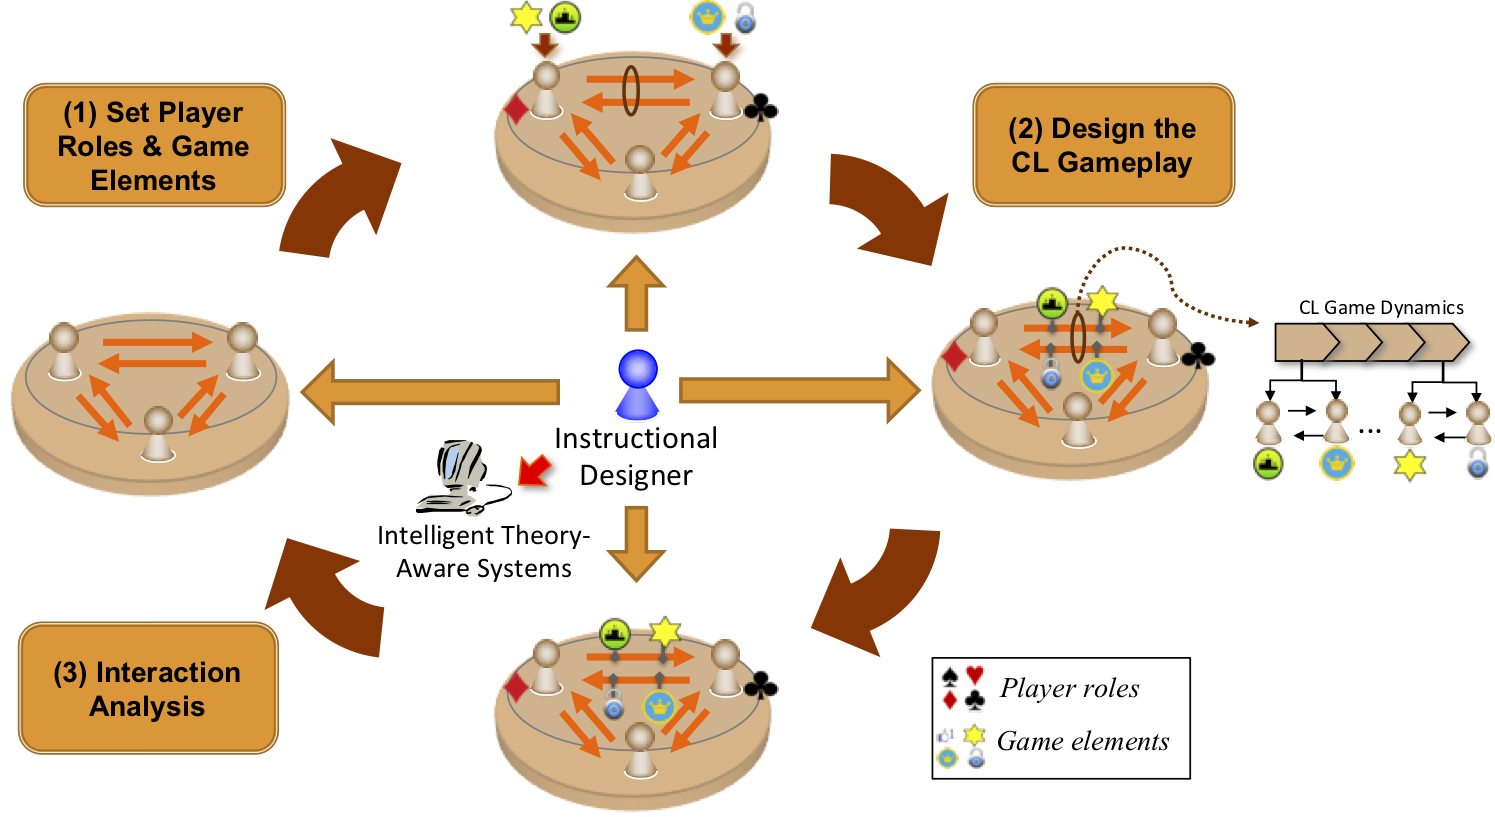
\includegraphics[width=1\textwidth]{images/chap-mechanisms-procedures/conceptual-flow-gamify-cl-sessions.png}
  \fautor
\end{figure}

Therefore, the basic stages to be accomplished in the conceptual flow to gamify CL sessions by intelligent-theory aware systems are:

\begin{description}
\item[Stage (1):] to set \emph{player roles} and \emph{game elements} for each participant in the CL session,
\item[Stage (2):] to design the \emph{CL gameplay} for the CL session, and
\item[Stage (3):] to perform an \emph{interaction analysis} over the obtained gamified CL sessions.
\end{description}

\subsection{Stage (1): Set Player Roles \& Game Elements}

For each participant in the CL session, using the information extracted from the ontology OntoGaCLeS, the task to gamify CL sessions should set the player roles and game elements to solve the context-dependency of gamification related to the participants' individual traits and characteristics.
In the ontology OntoGaCLeS, this information has been encoded as models to personalize gamification in CL scenarios based on player types models (\autoref{chapter:ontogacles-1}).
Based on these model, ontological structures to represent gamified CL scenarios (\autoref{subsec:gamified-cl-scenario} are used as a source of information by an intelligent-theory aware to give suggestions about the player roles and game elements that would be assigned for the participants of a CL session.

Having a set of ontological structures to represent CL scenarios in the variable \aspas{$ontModel$} as an ontology-based model to personalize the gamification in CL scenarios, the \autoref{algorithm:set-player-roles-and-game-elements} is a procedure to obtain a map of player roles and participants in the array \aspas{$playerRoles$,} where the keys represent the player roles and the values for the element \aspas{$playerRoles[pr]$} are lists of participants that will be play the player role \aspas{$pr$}. The procedure also establishes in the array \aspas{$gameElements$} a map between the player roles (\emph{keys}) and game elements (\emph{values}) that will be employed to motivate the participants of these player roles.

The steps of \autoref{algorithm:set-player-roles-and-game-elements} in a narrative form is described as follows:

\begin{enumerate}
\item From \aspas{\emph{an ontology-based model to personalize gamification in CL scenarios based on player types models}} ($ontModel$), the algorithm selects a subset of gamified CL scenarios ($scenarios$) that
would lead the participants (\emph{CL role holders}) from a CL session \aspas{$s$} to attain individual motivational goals defined in the motivational strategies. This first step is accomplished by calling the function \aspas{\emph{selectGamifiedCLSessionFor}($ontModel$, $s$)} (line 2).

\item Having the set of gamified CL scenarios \aspas{$scenarios$,} the algorithm checks the necessary conditions to
assign the player roles for the CL role holders who have the potential to become player role holders in each gamified CL scenario ($g \in scenarios$), and a priority queue \aspas{$q$} is established based on the number of participants that could be assigned for the \emph{I-Player role} and the number of desired conditions that are satisfied. This second step is carried out by the function \aspas{\emph{priorityQueueByPlayerRoles}($scenarios$, $s$)} (line 3).

\item The algorithm sets the player roles for the CL role holders if no one restriction is violated in the motivational strategy (\emph{Y<=I-mot goal}) of a gamified CL scenario \aspas{$g$} with highest priority in the queue \aspas{$q$.} In this sense, the loop \aspas{\emph{while}} (lines 6-24) iterates through the queue \aspas{$q$} searching the gamified CL scenario \aspas{$g$} with highest priority and without any violated restriction. In this scenario \aspas{$g$,} the participants for the player roles are defined as role holders of \emph{I-Player role} in the motivational strategies, and they are extracted in the array \aspas{$playerRoles[ms]$} through the loop \aspas{\emph{for}} (lines 25-30). 

\item Finally, the algorithm sets the proper game elements for the CL role holders using the structure \aspas{\emph{Gameplay strategy}} (\emph{I-gameplay}). This step is accomplished by setting the constraints \aspas{\emph{What to use}} into the array \aspas{$gameElements[rh]$} for the role holders \aspas{$rh$} defined as constraints in the roles \aspas{\emph{Primary focus (P)}} (lines 32-42).
\end{enumerate}

\begin{algoritmo}
\caption{Algorithm to set player roles and game elements in a CL session \aspas{$s$}}
\label{algorithm:set-player-roles-and-game-elements}
\begin{algorithmic}[1]\small
\Procedure{setPlayerRolesAndGameElements}{$ontModel$, $s$}
  \State $scenarios \gets$ \Call{selectGamifiedCLSessionsFor}{$ontModel$, $s$}
  \State $q \gets$ \Call{priorityQueueByPlayerRoles}{$scenarios$, $s$}
%  \LeftComment{Setting player roles if no one restriction is violated in the ind. mot. strategies}
  \State $g \gets$ null
  \State $playerRoles \gets []$
  \While{$\neg$ \Call{isEmpty}{$q$} $\land$ $g = null$}
    \State $iRHs, youRHs \gets []$
    \State $g \gets$ \Call{pullHighestPriorityElement}{$q$}
    \ForAll{$ms \in$ \Call{inhRolesOf}{\aspas{Motivational strategy}, $g$}}
      \ForAll{$p \in$ \Call{rolePlayingThingsFor}{\aspas{CL Role Holder}, $s$}}
        \State $pr \gets$ \Call{getBestPlayerRole}{$p$, $s$, $ms$}
        \If{$pr \in$ \Call{inhRolesOf}{\aspas{I-Player role}, $ms$}}
          $iRHs[ms] \gets iRHs[ms] \cup \{p\}$
        \EndIf
        \If{$pr \in$ \Call{inhRolesOf}{\aspas{You-Player role}, $ms$}}
          $youRHs[ms] \gets youRHs[ms] \cup \{p\}$
        \EndIf
      \EndFor
      \State $iSize \gets$ \Call{size}{$iRHs[ms]$}
      \State $youSize \gets$ \Call{size}{$youRHs[ms]$}
      \State $(iMin,iMax) \gets$ getMinMaxCard(\Call{inhRolesOf}{\aspas{I-Player role}, $ms$})
      \State $(youMin,youMax) \gets$ getMinMaxCard(\Call{inhRolesOf}{\aspas{You-Player role}, $ms$})
      \If{$iSize<iMin \lor iSize>iMax \lor youSize<youMin \lor youSize>youMax$}
        $g \gets null$
      \EndIf
    \EndFor
  \EndWhile
  \If{$g \neq null$}
    \ForAll{$ms \in$ \Call{inhRolesOf}{\aspas{Motivational strategy}, $g$}}
      \State $rh \gets$ \Call{roleHolderOf}{\aspas{I-Player role}, $ms$}
      \State $playerRoles[rh] \gets playerRoles[rh] \cup iRHs[ms]$
    \EndFor
  \EndIf
  \State $gameElements \gets []$
  \If{$g \neq null$}
    \ForAll{$indGameplay \in$ \Call{inhRolesOf}{\aspas{Gameplay strategy}, $g$}}
      \ForAll{$primaryFocus \in$ \Call{inhRolesOf}{\aspas{Primary focus (P)}, $indGameplay$}}
        \ForAll{$rh \in$ \Call{constrsOf}{$primaryFocus$}}
          \ForAll{$whatToUse \in$ \Call{inhRolesOf}{\aspas{What to use}, $indGameplay$}}
            \State $gameElements[rh] \gets gameElements[rh] \cup$ \Call{constrsOf}{$whatToUse$}
          \EndFor
        \EndFor
      \EndFor
    \EndFor
  \EndIf
\EndProcedure
\end{algorithmic}
\end{algoritmo}


To gather information from the ontology OntoGaCLeS, the \autoref{algorithm:set-player-roles-and-game-elements} and all the algorithms presented in this chapter hereafter have been developed using the basic functions shown in \autoref{qua:basic-functions-to-gather-information-from-ontogacles}.
In these functions, the ontological structures have been formalized as the logic primitives: $context(x)$, $roleHolder(rh)$, $roleConcept(r)$, $heldBy(r,rh)$, $dependsOn(r,x)$, $plays(x,r)$, $subClassOf(x,y)$, and $type(x,y)$; where the predicate symbols correspond to properties used by the Hozo editor to export an ontology based on the model of roles into OWL format as detailed in \cite{KozakiSunagawaKitamuraMizoguchi2007}.

\begin{quadro}[htb]
\caption{Basic functions to gather information from the ontology OntoGaCLeS}
\label{qua:basic-functions-to-gather-information-from-ontogacles}
\centering
\footnotesize
\begin{tabular}{|p{15cm}|}

\toprule
\textbf{inhRolesOf($roles$, $ctx$)} returns the unification of variable $ir$ for the roles $r \in roles$ and contexts $x \in ctx$ in the rules:  \\
$inheritedRoleOf(ir,r,x) \implies roleConcept(r), context(x), subClassOf(ir,r), dependsOn(r,x).$\\
$inheritedRoleOf(ir,r,x) \implies \exists r1; subClass(r1,r), inheritedRole(ir,r1,x).$\\

\hrule
\textbf{constraintConceptsFor($roles$, $ctx$)} returns the unification of variable $c$ for the roles $r \in roles$ and contexts $x \in ctx$ in the rules:\\
$constraintConceptFor(c,r,x) \implies context(x), plays(c,r), dependsOn(r,x).$\\
$constraintConceptFor(c,r,x) \implies \exists sr; subClass(sr,r), constraintConcept(c,sr,x).$\\

\hrule
\textbf{rolePlayingThingsFor($rhs$, $ctx\_ins$)} returns the unification of variable $i$ for the role holders $rh \in rhs$ and contexts instances $xi \in ctx\_ins$ in the rules:\\
$rolePlayingThingFor(i,rh,xi) \implies \exists ri,r; dependsOn(ri,xi), type(ri,r), heldBy(r,rh), roleHolder(rh),$ $plays(i,ri).$\\
$rolePlayingThingFor(i,rh,xi) \implies \exists xi1; dependsOn(xi1, xi), rolePlayingThingFor(i,rh,xi1).$\\


\hrule
\textbf{wholeConceptFromRole($r$)} returns the unification of variable $wc$ for the role $r$ in the rules:\\
$wholeConceptFromRole(wc,x) \implies \neg roleConcept(x), context(x).$\\

\hrule
\textbf{subConcepts($x$)} returns the unification of variable $s$ for the element $x$ in the rules:\\
$isA(s,x) \implies subClassOf(s,x).$\\
$isA(s,x) \implies \exists s1; subClassOf(s,s1), isA(s1,x).$\\


\hrule
\textbf{insByRolePlayingThings($x$, $params$)} returns the instances of context $x$ whose elements result from the intersection of all values in the dictionary $(r,vi) \in params$ when the variable $xi$ is unified in the rules:\\
$insByRolePlayingThing(xi,x,r,vi) \implies \exists ri;
context(x), type(xi,x), dependsOn(ri,xi), type(ri,r), plays(vi,ri).$\\




%$insByRolePlayingThing(xi,x,r,vi) \implies \exists ri,ri1,rhi;

%type(xi,x),

%plays(xi,ri1), 


%dependsOn(ri,ri1),
%type(ri,r),

%plays(vi,ri), type(ri,r), dependsOn(ri, x1)


%type(xi,x), type(ri,r),


%plays(vi,ri1), heldBy(ri1,rhi),
%plays(rhi,ri), dependsOn(ri,xi), type(xi,x), type(ri,r), dependsOn(r,x).$\\

%$insByRolePlayingThing(xi,x,r,vi) \implies \exists ri1;
%subClassOf(r1,r),
%insByRolePlayingThing(xi,x,r,vi).$\\


\bottomrule
\end{tabular}
 \fautor
\end{quadro}


In the following subsections, the steps of the \autoref{algorithm:set-player-roles-and-game-elements} are detailed using \autoref{tab:information-exemplify-attribution-player-roles-game-elements} as source of information to set the proper player roles and game elements for the participants of CL sessions: $s1$, $s2$, $s3$, and $s4$.
In this example, the ontology-based model to personalize gamification \aspas{$ontModel$} employed by the algorithm is a Bartle-based model shown in \autoref{fig:ontological-structures-bartle-based-model}, and it is constituted by the ontological structures: \emph{Gamified CL Scenario for Achievements}, \emph{Gamified CL Scenario for Exploration}, \emph{Gamified CL Scenario for Socialization}, and \emph{Gamified CL Scenario for Killers}.


\setlongtables{\small
\begin{longtable}{clllc}
\caption{Information used to exemplify the attribution of player roles and game elements in CL sessions}
\tabularnewline
\hline\hline
\multicolumn{1}{c}{Participant ID}&\multicolumn{1}{c}{Mot. Stage}&\multicolumn{1}{c}{Game style preference}&\multicolumn{1}{c}{Need state}&\multicolumn{1}{c}{CL Session ID}\tabularnewline
\hline
\endfirsthead\caption[]{\em (continued)} \tabularnewline
\hline
\multicolumn{1}{c}{Participant ID}&\multicolumn{1}{c}{Mot. Stage}&\multicolumn{1}{c}{Game style preference}&\multicolumn{1}{c}{Need state}&\multicolumn{1}{c}{CL Session ID}\tabularnewline
\hline
\endhead
\hline
\endfoot
\label{tab:information-exemplify-attribution-player-roles-game-elements}
p1 & amotivation & acting-orientation & mastery & s1\tabularnewline
p2 & amotivation & acting-orientation & mastery & s1\tabularnewline
p3 & amotivation & acting-orientation & mastery & s2\tabularnewline
p4 & amotivation & acting-orientation & mastery & s2\tabularnewline
p5 & amotivation & acting-orientation & mastery & s2\tabularnewline
p6 & amotivation & acting-orientation & mastery & s3\tabularnewline
p7 & amotivation & acting-orientation & mastery & s3\tabularnewline
p8 & amotivation & acting-orientation & mastery & s4\tabularnewline
p9 & amotivation & acting-orientation & mastery & s4\tabularnewline
p10 & amotivation & acting-orientation & mastery & s4\tabularnewline
\hline
\end{longtable}}

\begin{figure}[htb]
  \caption{Ontological structures to represent gamified CL scenarios in a Bartle-based model used to exemplify the attribution of player roles and game elements in CL sessions}
  \label{fig:ontological-structures-bartle-based-model}
  \centering
 % \includegraphics[width=1\textwidth]{images/chap-mechanisms-procedures/ontological-structures-bartle-based-model.png}
  \fautor
\end{figure}

\subsubsection*{Step 1: Selecting the gamified CL scenarios that would lead the participants to attain the individual motivational goals defined in the motivational strategies}

This step is accomplished by the function \aspas{\emph{selectGamifiedCLSessionFor}($ontModel$, $s$)} detailed in the \autoref{algorithm:select-gamified-cl-scenarios-for}. The pseudo-code iterates in each motivational strategies \aspas{$ms$} (lines 4-13), and its verifies that there is a potential player \aspas{$p$} for the \aspas{I-player role} to achieve the individual motivational goals defined in the motivational  \aspas{$ms$} (lines 6-11).
The potential players for the \aspas{I-player role} are indicated as constraints of its role in each motivational strategy of the ontological structure to represent gamified CL scenarios, thereby the function \aspas{\emph{constrsOf}($iPlayerRole$)} (line 6) obtains the class of CL role holders, and the function \aspas{\emph{insOfRoleHoldersIn}($clRoleHolder$, $s$)} (line 7) obtains the participants that become CL role holders in the CL session \aspas{$s$.}
Finally, the function \aspas{\emph{canAchieveIndMotGoalsOf}($p$, $s$, $ms$)} (line 8) verifies if the individual motivational goals defined in the motivational strategy \aspas{$ms$} can be achieved by some participant \aspas{$p$} of the CL session \aspas{$s$,} and when this condition is satisfied, the gamified CL scenario \aspas{$g$} is added to the variable \aspas{\emph{set}} that is returned at the end of function (line 15).

\begin{algoritmo}
\caption{Algorithm to select the gamified CL scenarios that would lead the participants of a CL session \aspas{$s$} to achieve their individual mot. goals from an ontology-based model \aspas{$ontModel$}}
\label{algorithm:select-gamified-cl-scenarios-for}
\begin{algorithmic}[1]\small
\Function{selectGamifiedCLSessionsFor}{$ontModel$, $s$}
  \State $set \gets \emptyset$
  \ForAll{$g \in ontModel$}
    \ForAll{$ms \in$ \Call{inhRolesOf}{\aspas{Motivational strategy}, $g$}}
      \ForAll{$iPlayerRole \in$ \Call{inhRolesOf}{\aspas{I-Player role}, $ms$}}
        \ForAll{$clRoleHolder \in$ \Call{constrsOf}{$iPlayerRole$}}
          \ForAll{$p \in$ \Call{insOfRoleHolderIn}{$clRoleHolder$, $s$}}
            \If{\Call{canAchieveIndMotGoalsOf}{$p$, $s$, $ms$}}
              $set \gets set \cup \{g\}$
            \EndIf
          \EndFor
        \EndFor
      \EndFor
    \EndFor
  \EndFor
  \State \Return $set$
\EndFunction
\end{algorithmic}
\end{algoritmo}

The pseudo-code for the function \aspas{\emph{canAchieveIndMotGoalsOf}($p$, $s$, $ms$)} is detailed in \autoref{algorithm:can-achieve-ind-mot-goals-of}, and it returns true when the participant \aspas{$p$} of a CL session \aspas{$s$} can achieve the individual motivational goals indicated in the motivational strategy \aspas{$ms$.} This verification is done by checking out that the participant \aspas{$p$} is the \emph{holder} of initial stages defined in the individual motivation goals of motivational strategy \aspas{$ms$.} Thus, the function \aspas{\emph{insByRolePlayingThings}} (line 2) obtains the current motivational stages that are holden by the participant \aspas{$p$} in reference to the CL session \aspas{$s$.} If there is no information about these stages in the knowledge base, the algorithm returns $true$ (line 23) assuming that the motivational strategy \aspas{$ms$} can lead the participant \aspas{$p$} to attain the individual motivational goals indicated by it. If the number of individual motivational goals \aspas{$nIndMotGoals$} that can be achieved by the participant \aspas{$p$} is not equal to the number of individual motivational goals indicated in the motivational strategy, the function returns $false$ (line 20). To validate if an individual motivational goal \aspas{$indMotGoal$} can be attained by a participant \aspas{$p$,} the functions \aspas{\emph{inhRolesOf}(\aspas{init stage}, $indMotGoal$)} (line 8) and \aspas{\emph{constrsOf}($initStageRole$)} (line 9) obtain the initial stages for this goal, and the loop \aspas{\emph{for}} (line 10-13) iterates in the current motivational stages of the participant \aspas{$p$} verifying that he/she holds this stage by the function \aspas{\emph{isA}($pStage$, $initStage$)} (line 11).

\begin{algoritmo}
\caption{Algorithm to verify if a participant \aspas{$p$} of a CL session \aspas{$s$} can achieve the individual motivational goals defined in the motivational strategy \aspas{$ms$}}
\label{algorithm:can-achieve-ind-mot-goals-of}
\begin{algorithmic}[1]\small
\Function{canAchieveIndMotGoalsOf}{$p$, $s$, $ms$}
  \State $pStages \gets$ \Call{insByRolePlayingThings}{\aspas{Motivational stage}, \{(\aspas{holder},$p$), (\aspas{target},$s$)\}}
  \If{$pStages \neq \emptyset$}
    \State $nIndMotGoals \gets 0$
    \ForAll{$indMotGoalRole \in$ \Call{inhRolesOf}{\aspas{I-mot goal (I)}, $ms$}}
      \State $canAchieve \gets false$
      \ForAll{$indMotGoal \in$ \Call{constrsOf}{$indMotGoalRole$}}
        \ForAll{$initStageRole \in$ \Call{inhRolesOf}{\aspas{init stage}, $indMotGoal$}}
          \ForAll{$initStage \in$ \Call{constrsOf}{$initStageRole$}}
            \ForAll{$pStage \in pStages$}
              \If{\Call{isA}{$pStage$, $initStage$}} $canAchieve \gets true$
              \EndIf
            \EndFor
          \EndFor
        \EndFor
      \EndFor
      \If{$canAchieve$} $nIndMotGoals \gets nIndMotGoals + 1$
      \EndIf
    \EndFor
    \If{$nIndMotGoals \neq$ size(\Call{inhRolesOf}{\aspas{I-mot goal (I)}, $ms$})} \Return $false$
    \EndIf
  \EndIf
  \State \Return $true$
\EndFunction
\end{algorithmic}
\end{algoritmo}

\subsubsection*{Step 2: Setting a priority queue for the gamified CL scenarios based on the necessary and desired conditions that are satisfied by the participants to become player roles}

\autoref{algorithm:set-priority-queue-by-player-roles} shows the pseudo-code for the function \aspas{\emph{priorityQueueByPlayerRoles}} that establishes a priority queue \aspas{$q$} for the gamified CL scenarios indicated in the set \aspas{$scenarios$.} The priority queue is based on the necessary and desired conditions that are satisfied by the participants of a CL session \aspas{$s$} to become player roles indicated as \emph{I-Player role} in the motivational strategies. Thus, the loop \aspas{\emph{for}} (lines 5-19) iterates in the motivational strategies of gamified CL scenario \aspas{$g$,}  the loop \aspas{\emph{for}} (lines 6-18) iterates in the \emph{I-Player role}, the loop \aspas{\emph{for}} (lines 7-17) iterates in the constraints of \emph{I-Player role}, and the loop \aspas{\emph{for}} (lines 8-16) iterates in the participants that have the potential to play the \emph{I-Player role}. When one of these participants indicated in the variable \aspas{$p$} can achieve the individual motivational goals of the motivational strategy by the function \aspas{\emph{canAchieveIndMotGoalsOf}($p$, $ms$)} (line 9), and there is a player role as whole concept \aspas{$wcPlayerRole$} in which the participant \aspas{$p$} satisfies the necessary conditions obtained by the function \aspas{\emph{satisfyNecessaryConditions}($p$, $iPlayerRole$, $s$)} (line 10), the algorithm indicates that he/she can play the \emph{I-Player role} by increasing the number of participants to play an \emph{I-Player role} \aspas{$n$} by one (line 12). The number of desired conditions \aspas{$d$} that are satisfied by the participant \aspas{$p$} is calculated by the function \aspas{\emph{noSatisfiedDesiredConditions}($p$, $wcPlayerRole$, $s$)} (line 13). Finally, if there is a participant that can play the \emph{I-Player role} in some motivational strategy, the gamified CL scenario \aspas{$g$} is inserted in the queue \aspas{$q$} with the priority pair <$n,d$> (line 20).

\begin{algoritmo}
\caption{Algorithm to set a priority queue for the gamified CL \aspas{$scenarios$} according to the conditions that are satisfied by the participants of a CL session \aspas{$s$} to become player roles}
\label{algorithm:set-priority-queue-by-player-roles}
\begin{algorithmic}[1]\small
\Function{priorityQueueByPlayerRoles}{$scenarios$, $s$}
  \State $q \gets []$
  \ForAll{$g \in scenarios$}
    \State $n, d \gets 0$
    \ForAll{$ms \in$ \Call{inhRolesOf}{\aspas{Motivational Strategy}, $g$}}
      \ForAll{$iPlayerRole \in$ \Call{inhRolesOf}{\aspas{I-Player role}, $ms$}}
        \ForAll{$clRoleHolder \in$ \Call{constrsOf}{$iPlayerRole$}}
          \ForAll{$p \in$ \Call{insOfRoleHolderIn}{$clRoleHolder$, $s$}}
            \If{\Call{canAchieveIndMotGoalsOf}{$p$, $ms$}}
              \State $wcPlayerRole \gets$ \Call{satisfyNecessaryConditions}{$p$, $iPlayerRole$, $s$}
              \If{$wcPlayerRole \neq null$}
                \State $n \gets n+1$
                \State $d \gets d+$\Call{noSatisfiedDesiredConditions}{$p$, $wcPlayerRole$, $s$}
              \EndIf
            \EndIf
          \EndFor
        \EndFor
      \EndFor
    \EndFor
    \If{$n > 0$} \Call{insertWithPriority}{$q$, $g$, <$n,d$>}
    \EndIf
  \EndFor
  \State \Return $q$
\EndFunction
\end{algorithmic}
\end{algoritmo}

The function \aspas{\emph{satisfyNecessaryConditions}} detailed by the pseudo-code shown in \autoref{algorithm:satisfy-necessary-conditions} returns the player role as a whole concept when all its necessary conditions are satisfied by the participant \aspas{$p$} of a CL session \aspas{$s$}. Thus, the function \emph{roleAsWholeConcept} (line 2) obtains the player role as a whole concept, and the current psychological need states \aspas{$pNeedStates$,} individual personality trait states \aspas{$pTraitStates$} and motivation states \aspas{$pMotStates$} for the participant \aspas{$p$} is obtained by the function \emph{insByRolePlayingThings} (line 3-5). Having these states the loop \aspas{\emph{for}} (line 6-31), the algorithm iterates in the subconcepts of player role as a whole concept, and when all the necessary conditions of this player role or any subconcept are satisfied by the participant, the algorithm returns this concept (line 28-29). The subconcepts of a player role as whole concept in the ontology OntoGaCLeS represent alternative forms to represent the same player role. All the condition of a player role as whole concept are satisfied when the number of conditions \aspas{$c$} satisfied by the participant \aspas{$p$} is the same that the number of necessary conditions defined in the player role (line 28). The loop \aspas{\emph{for}} (lines 8-27) iterates in the necessary conditions of player role, and the loop \aspas{\emph{for}} (lines 10-23) iterates in the constraints of these conditions to check if the participant \aspas{$p$} satisfies the condition \aspas{$cond$.} This condition is satisfied when there is no information related to the participant's state and the condition (line 17) or when one of the participant's states is instance of condition state (line 20). The checking of this condition is accomplished by the loop \aspas{\emph{for}} (lines 19-22).

\begin{algoritmo}
\caption{Algorithm to returns player role \aspas{$pr$} as a whole concept if the participant \aspas{$p$} of a CL session \aspas{$s$} satisfies all necessary conditions to play this player role}
\label{algorithm:satisfy-necessary-conditions}
\begin{algorithmic}[1]\small
\Function{satisfyNecessaryConditions}{$p$, $pr$, $s$}
  \State $wcPlayerRole \gets$ \Call{roleAsWholeConcept}{$pr$}
  \State $pNeedStates \gets$ \Call{insByRolePlayingThings}{\aspas{Psychological need state},\{(\aspas{holder},$p$)\}}
  \State $pTraitStates \gets$ \Call{insByRolePlayingThings}{\aspas{Ind. personality trait state},\{(\aspas{holder},$p$)\}}
  \State $pMotStates \gets$ \Call{insByRolePlayingThings}{\aspas{Motivation state},\{(\aspas{holder},$p$),(\aspas{target},$s$)\}}  
  \ForAll{$wcPlayerRole \in$ \Call{subConceptsOf}{$wcPlayerRole$} $\cup \{wcPlayerRole\}$}
    \State $c \gets 0$
    \ForAll{$condRole \in$ \Call{inhRolesOf}{\aspas{Necessary condition}, $wcPlayerRole$}}
      \State $isSatisfied \gets false$
      \ForAll{$cond \in$ \Call{constrsOf}{$condRole$}}
        \If{\Call{isA}{$cond$, \aspas{Motivation state}}} $pStates \gets pMotStates$
        \EndIf
        \If{\Call{isA}{$cond$, \aspas{Psychological need state}}} $pStates \gets pNeedStates$
        \EndIf
        \If{\Call{isA}{$cond$, \aspas{Ind. personality trait state}}} $pStates \gets pTraitStates$
        \EndIf
        \If{$pStates = \emptyset$} $isSatisfied \gets true$
        \Else
          \ForAll{$pState \in pStates$}
            \If{\Call{isA}{$pState$,$cond$}} $isSatisfied \gets true$
            \EndIf
          \EndFor
        \EndIf
      \EndFor
      \If{$isSatisfied$} $c \gets c+1$
      \EndIf
    \EndFor
    \If{$c>0 \land c =$ size(\Call{inhRolesOf}{\aspas{Necessary condition}, $wcPlayerRole$})}
      \State \Return $wcPlayerRole$
    \EndIf
  \EndFor
  \State \Return $null$
\EndFunction
\end{algorithmic}
\end{algoritmo}

To count the number of satisfied desired conditions, the algorithm to set a priority queue for the gamified CL scenarios employs the function \aspas{\emph{noSatisfiedDesiredConditions}} whose pseudo-code is detailed in the \autoref{algorithm:no-satisfied-desired-conditions}. This pseudo-code is similar to the pseudo-code of the function \aspas{\emph{satisfyNecessaryConditions},} but with the difference that it does not iterate in the subconcepts of player role and the value returned by it is not true or false, the algorithm return the number of desired conditions that are satisfied by the participant.

\begin{algoritmo}
\caption{Algorithm to count the number of satisfied desired conditions for a participant \aspas{$p$} of a CL session \aspas{$s$} playing the player role \aspas{$wcPlayerRole$}}
\label{algorithm:no-satisfied-desired-conditions}
\begin{algorithmic}[1]\small
\Function{noSatisfiedDesiredConditions}{$p$, $wcPlayerRole$, $s$}
  \State $d \gets 0$
  \State $pNeedStates \gets$ \Call{insByRolePlayingThings}{\aspas{Psychological need state},\{(\aspas{holder},$p$)\}}
  \State $pTraitStates \gets$ \Call{insByRolePlayingThings}{\aspas{Ind. personality trait state},\{(\aspas{holder},$p$)\}}
  \State $pMotStates \gets$ \Call{insByRolePlayingThings}{\aspas{Motivation state},\{(\aspas{holder},$p$),(\aspas{target},$s$)\}}
  \ForAll{$condRole \in$ \Call{inhRolesOf}{\aspas{Desired condition}, $wcPlayerRole$}}
    \State $isSatisfied \gets false$
    \ForAll{$cond \in$ \Call{constrsOf}{$condRole$}}
      \If{\Call{isA}{$cond$, \aspas{Motivation state}}} $pStates \gets pMotStates$
      \EndIf
      \If{\Call{isA}{$cond$, \aspas{Psychological need state}}} $pStates \gets pNeedStates$
      \EndIf
      \If{\Call{isA}{$cond$, \aspas{Ind. personality trait state}}} $pStates \gets pTraitStates$
      \EndIf
      \If{$pStates = \emptyset$} $isSatisfied \gets true$
      \Else
        \ForAll{$pState \in pStates$}
          \If{\Call{isA}{$pState$,$cond$}} $isSatisfied \gets true$
          \EndIf
        \EndFor
      \EndIf
    \EndFor
    \If{$isSatisfied$} $d \gets d+1$
    \EndIf
  \EndFor
  \State \Return $d$
\EndFunction
\end{algorithmic}
\end{algoritmo}

\subsubsection*{Step 3: Setting player roles if no one restriction is violated in the motivational strategy}



 which all necessary 

This player role is returned  


 where the keys represent the player roles and the values for the element \aspas{$playerRoles[pr]$} are lists of participants to be assigned for the player role \aspas{$pr$}

The highest gamified CL scenario is extracted from the queue \aspas{$q$} by the function \aspas{\emph{pullHighestPriorityElement}($q$)} (line 8). When the number of role holders for the \emph{I-Player role} in the variable \aspas{$iSize$} or the number of role holders for the \emph{You-Player role} in the variable \aspas{$youSize$} are outside of the limits indicated by the cardinality of the roles, the constraints in the motivational strategy \aspas{$ms$} is violated. The role holders for the \emph{I-Player role} and \emph{You-Player role} are determined in the variables \aspas{$iRHs$} and \aspas{$youRHs$} through the loop \aspas{\emph{For}} (lines 10-16), where the best player role \aspas{$pr$} for a participant \aspas{$p$} in a CL session \aspas{$s$} according to the motivational strategy \aspas{$ms$} is obtained by the function \aspas{\emph{getBestPlayerRole}($p$, $s$, $ms$)} (line 11).


%to set \emph{player roles} and \emph{game elements}

%CL scenarios to persuade the participants to follow the interactions defined by the sequencing mechanism of a CSCL
%script, computer-based mechanisms can be built to help the design of CL gameplay in gamified CL scenarios.

%The building of these structures to define an ontological model comprises the following steps: (1) to identify the
%player roles that can be assigned for the participants of CL scenario when they are playing a CL role, (2) to identify
%the restriction and elements of motivational strategies for each pair of identified player roles, and (3) to define
%individual gameplay strategies for the identified pairs of player roles.


\begin{algoritmo}
\caption{Algorithm to get the best player role to be assigned for a participant \aspas{$p$} in a CL session \aspas{$s$} according to a motivational strategy \aspas{$ms$}}
\label{algorithm:get-best-player-role}
\begin{algorithmic}[1]\small
\Function{getBestPlayerRole}{$p$, $s$, $ms$}
  \State $iPlayerRoles \gets$ \Call{inheritedRolesFor}{\aspas{I-Player role}, $ms$}
  \State $iConstraints \gets$ \Call{constraintConceptsFor}{$iPlayerRoles$}
  \State $iParticipants \gets$ \Call{rolePlayingThingsFor}{$iConstraints$, $s$}
  \State $youPlayerRoles \gets$ \Call{inheritedRolesFor}{\aspas{You-Player role}, $ms$}
  \State $youConstraints \gets$ \Call{constraintConceptsFor}{$youPlayerRoles$}
  \State $youParticipants \gets$ \Call{rolePlayingThingsFor}{$youConstraints$, $s$}
  \If{$p \in (iParticipants \setminus youParticipants)$}
    \State \Return \Call{satisfyNecessaryConditions}{$p$, $iPlayerRoles$, $s$}
  \ElsIf{$p \in (youParticipants \setminus iParticipants)$}
    \State \Return \Call{satisfyNecessaryConditions}{$p$, $youPlayerRoles$, $s$}
  \ElsIf{$p \in (iParticipants \cap youParticipants)$}
    \State $iPlayerRole \gets$ \Call{satisfyNecessaryConditions}{$p$, $iPlayerRoles$, $s$}
    \State $youPlayerRole \gets$ \Call{satisfyNecessaryConditions}{$p$, $youPlayerRoles$, $s$}
    \If{$iPlayerRole \neq null \land youPlayerRole \neq null$}
      \State $iNo \gets$ \Call{noSatisfiedDesiredConditions}{$p$, $iPlayerRole$, $s$}
      \State $youNo \gets$ \Call{noSatisfiedDesiredConditions}{$p$, $youPlayerRole$, $s$}
      \If{$iNo \geq youNo$} \Return $iPlayerRole$
      \ElsIf{$iNo < youNo$} \Return $youPlayerRole$
      \EndIf
    \ElsIf{$iPlayerRole \neq null$} \Return $iPlayerRole$
    \ElsIf{$youPlayerRole \neq null$} \Return $youPlayerRole$
    \EndIf
  \EndIf
  \State \Return $null$
\EndFunction
\end{algorithmic}
\end{algoritmo}


\subsection*{Step (2): Design the CL Gameplay}

By setting up the interactions between the selected game elements and the player role holders defined in the step (1),
the design of the \emph{CL gameplay} is carried out employing as source the information the gamified I\_L events defined
as necessary and desired interaction in the CL game dynamics (\emph{How to play}) of CL process refereed as \emph{CL
Gameplay} in the ontological structure to represent Gamified CL scenarios. For establishing the value of the game
rewards, during the setting of the interactions, the GMIF model can be employed as was detailed in \autoref{sec
:application-giving-rewards-by-gimf-model}.

For a gamified CL session instantiated from a CSCL scripts based on the Cognitive Apprenticeship theory, \autoref{fig
:design-cl-gameplay} exemplifies the design of a CL Gameplay for the interaction \aspas{\emph{Giving information}}
defined as \emph{instructional event}. Thus, before the instructional action, to persuade a master student to give
information, the interactions between the game element \aspas{\emph{Point-system (individual)}} and the master student
is defined as the game action \aspas{\emph{Promise points}} in the ontological structure, this game action is
implemented as the promise of points to elaborate the prob. list as shown in the the frame (a1), and the quantity of
points to be given to the master student after the execution of the instructional action \aspas{\emph{give information}}
is calculated by the GMIF model as was proposed in \autoref{sec:application-giving-rewards-by-gimf-model}. For the game
consequence event, as shown in the frame (a2), a 5-scale GMIF model has built employing 5-scale of challenge levels
(with +100 points to the 0:lowest level, +200 points to the 1:low level, +400 points to the medium level, +800 points to
the 3:high level, and +1000 points to the 4:highest level), so that the game reward to be given for the master student
after to perform the instructional action to maintain the flow state during the transition $s(3,y) \to s(4,y)$ should be
+1000 points as shown in frame (a3).

To persuade the master students to perform the instructional action, the game stimulus event in the ontological
structure defines the game action \aspas{\emph{Display/highlight current position}} as the game action that should be
performed by the game element \aspas{\emph{Leaderboard (individual ranking)}.} The implementation of this game action is
shown in the frame (b) of \autoref{fig:design-cl-gameplay}. The game action \aspas{\emph{Show condition to achieve the
next level}} defined as game stimulus event for the game element \aspas{\emph{Achievement system (participation level)}}
has been implemented as shown in the frame (c), in which the game action has been implemented by the message
\aspas{\emph{Level 06 of Participation: to attain 6400 points}.}

%\newpage \begin{figure}[htb]  \caption{Designing the CL Gameplay in the instructional event \aspas{\emph{Giving
%information}}}  \label{fig:design-cl-gameplay}  \centering  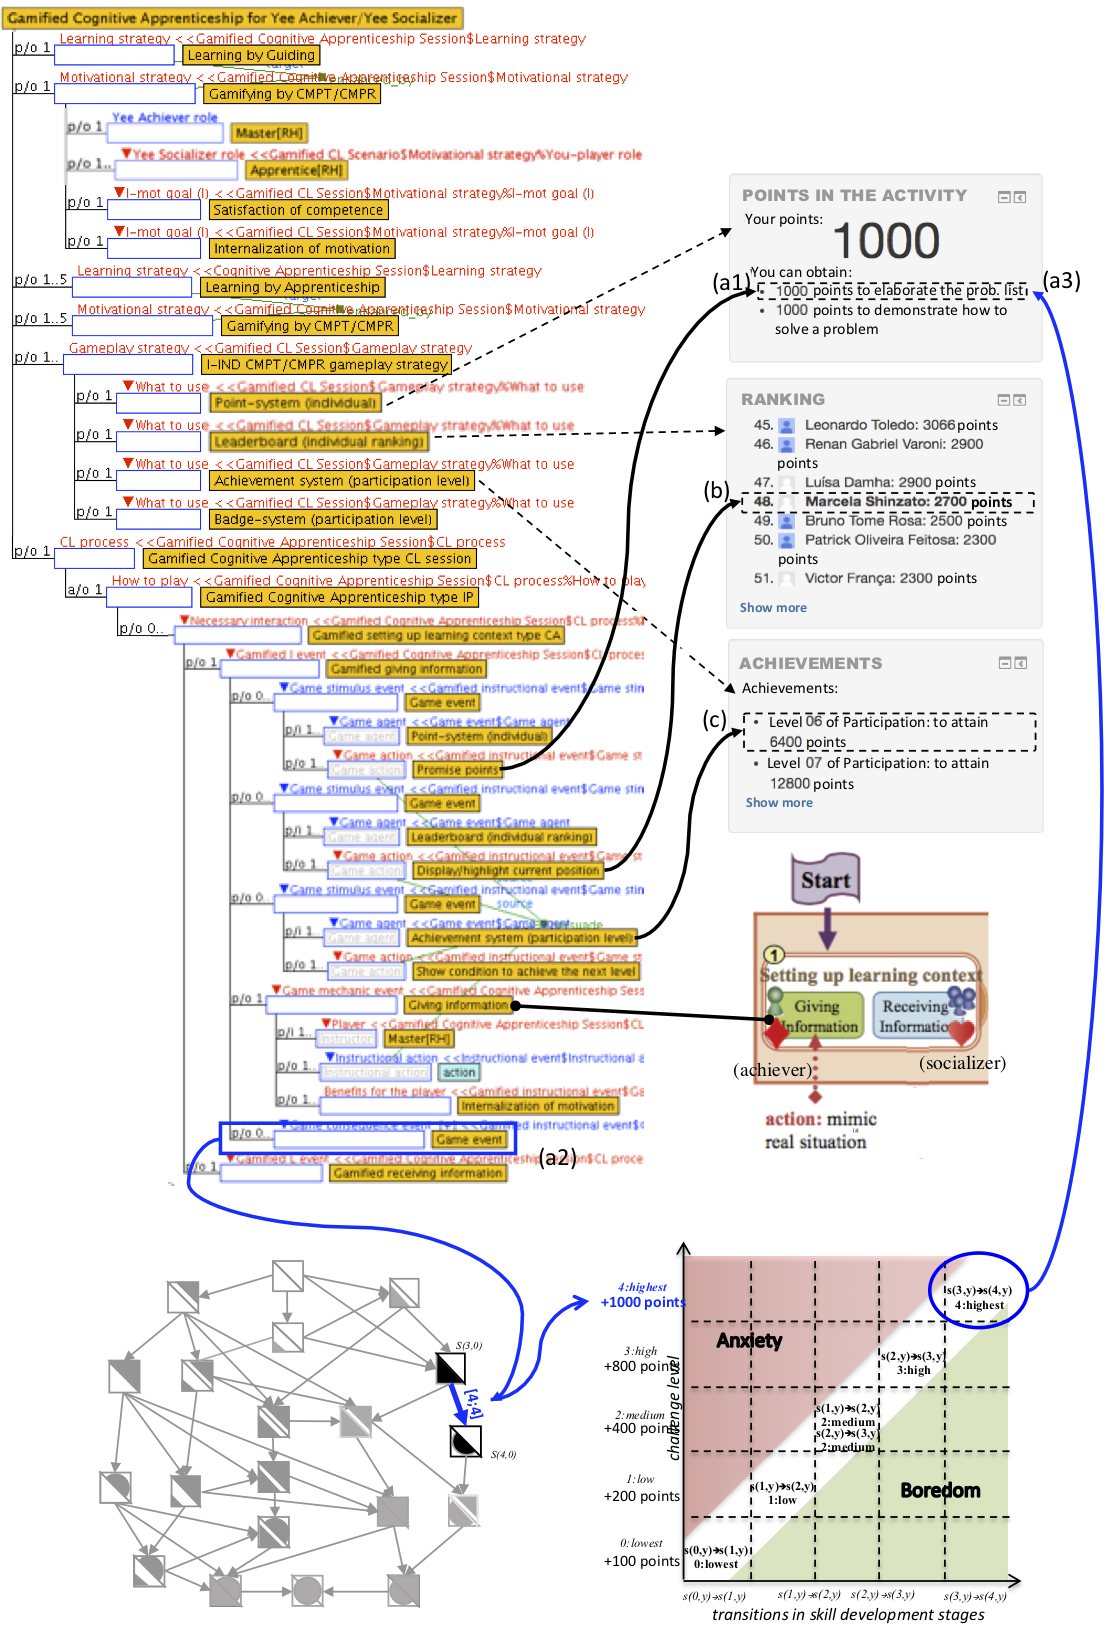
\includegraphics[width=0.8\textwidth]{images/chap-
%mechanisms-procedures/design-cl-gameplay.png}  \fautor \end{figure}

\newpage %As we mentioned in the previous section, persuasive game design models [24, 30] are the information source to
define the Gamified influential I\_L events in gamified CL scenarios. Currently, in the ontology OntoGaCLes, the
Persuasive Game Design Strategies (PGDSs) proposed by Orji et al. [24] have been applied in the CL process of CL
scenarios based on the Cognitive Apprentice theory, and these PGDSs have been personalized for achievers using the Yee’s
model. Fig 5(d) shows part of the ontological structure formalized using the PGDSs to represent the event “Gamified
setting up learning context” in which the instructional event “Gamified Giving information” has as stimulus three game
events defined for game actions: promise points, display/highlight current position, and show condition to achieve the
next level. These game actions are defined to persuade the master student to perform the instructional action “mimic
real situation” defined in the instructional event “Giving information.” Furthermore, the gamified I\_L event “Gamified
setting up learning context” defines that the game actions will be respectively done by the game agents: a point system
with individual points, a leaderboard with an individual ranking, and the achievement system for participation level.
Finally, the expected benefit for the master student is the internalization of motivation (benefits for the player) as
shown in Fig 5(d).

\subsection*{Step (3): Interaction Analysis}

Although the game elements are introduced and set-up in a CL session to to change peoples’ attitudes, intentions,
motivations and/or behaviors through the whole CL process, there is no guarantee that these change occurred during the
execution of gamifed CL sessions. Therefore, after the execution of a gamified CL session obtained by intelligent
theory-aware systems that uses the ontology OntoGaCLeS, it is necessary to understand what changes occurred while the
gamified CL scenario was executed in the learning environment. In this sense, an \emph{interaction analysis} should be
carried out with the data gathered from the virtual learning environment in which the gamified CL sessions was executed
to identify whether the designed changes occurred satisfactorily. To enable computers to support such a task, it is
necessary to use the ontological structures that represent the desired changes in the gamified I\_L events, and the
changes in real interactions. By doing so, computers can compare the difference between the changes indicated by the
ontological structures and the real interactions which helps to create a metric to measure the benefits of gamification
and to improve the modeling of gamified I\_L events.

%(2) Design the CL Gameplay

%In the step (1), the designer sets the proper player roles and game elements for each student. In the step (2), he/she
%designs the CL gameplay as a set of CL game dynamics employing the player roles and game elements that were setting in
%the first phase. Final-ly, in the step (3), the designer makes an interaction analysis over the obtained gamified CL
%scenarios to propose better solutions by the meaningful result obtained during the run-time of CSCL scripts.
 
%Fig.1. Flow to gamify a CL scenario in an intelligent theory-aware system. In previous works [2, 4, 5], we define
%ontological structures that allow us to accomplish the step (1) by the building of models that personalize gamification
%based on the individual differences of students, such as cur-rent motivation stages, psychological needs and individual
%personality preferences. To accomplish the step (2), the work [3] propose a set of ontological structures to represent
%the application of PSs in CL scenarios. To establish these structures employing concepts and semantic relations in our
%ontology, we use the ontology engineering techniques [24], the Hozo Ontology editor [21], and the model of roles
%proposed by Mizogu-chi, R. et al. [26].


% The ont-gamified CL sessions have been gamified according to the suggestions given by intelligent-theory aware
% systems, which in turn used the ontology OntoGaCLeS as information source to give these suggestions.

%\newpage %%%%%%%%%%%%%%%%%%%%%%%%%%%%%%%%%% \section[Reference Architecture of Intelligent-theory Aware
%Systems]{Reference Architecture of Intelligent-theory Aware Systems that Use the Ontology OntoGaCLeS} \label{sec
%:reference-architecture}

\autoref{fig:reference-architecture} shows the proposed reference architecture for building the next generation of
intelligent systems, referred to as intelligent theory-aware systems, that can be created and used to deal with the
motivation problem by the gamification of CL sessions. This reference architecture aims to help two stakeholders,
\emph{instructional designer} and emph{gamify expert}, to accomplish their activities in two different environments
denominated aspas{emph{Intelligent theory-aware authoring environment}} and aspas{emph{Gamification-framework editing
environment}.}

%\begin{figure}[htb]  \caption{A reference architecture of intelligent theory-aware systems to gamify CL sessions}
%\label{fig:reference-architecture}  \centering  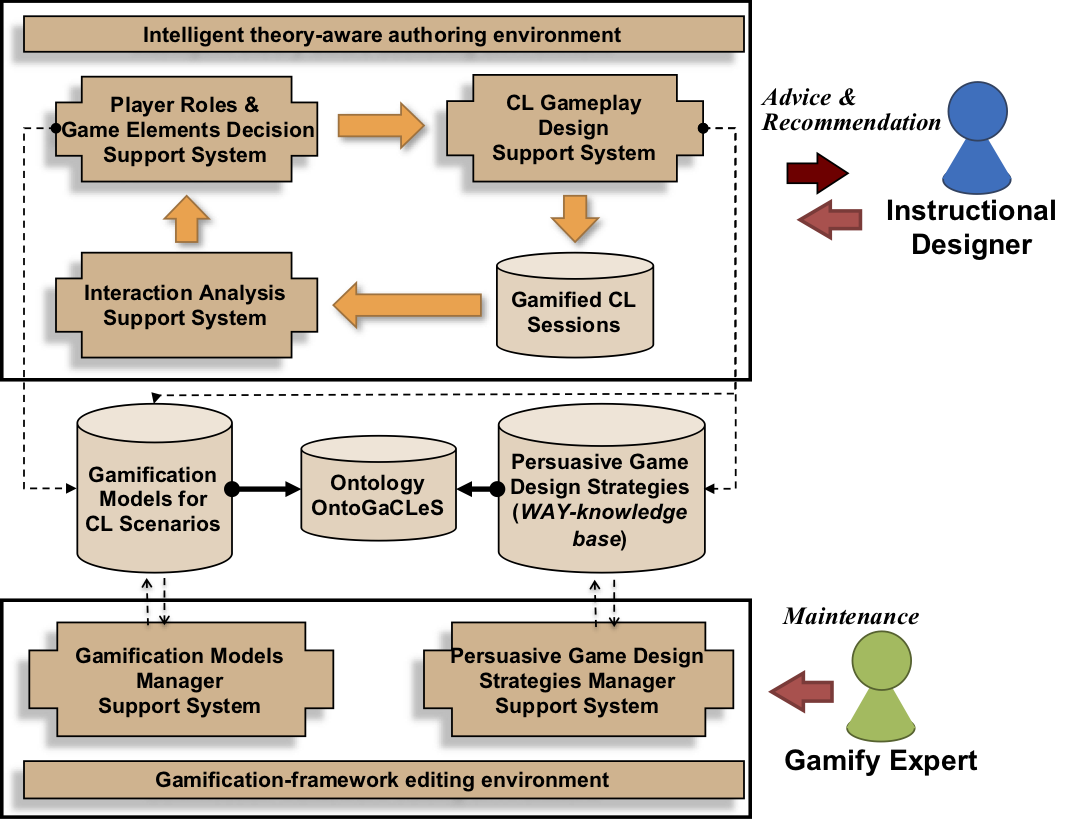
\includegraphics[width=1\textwidth]{images/chap-mechanisms-procedures
%/reference-architecture.png}  \fautor \end{figure}

\noindent textbf{Intelligent Theory-aware Authoring Environment}: An environment developed to provide advices and
recommendations to help the instructional designer to gamify CL sessions, so that it is composed by three intelligent
theory-aware systems, each one of them developed to support one of these step defined in the proposed conceptual flow
to gamify CL sessions (autoref{sec:conceptual-flow-gamify-cl-sessions}). In this sense, this environment is composed by
the following support-systems:
\begin{itemize}
\item A emph{Player Roles \& Game Elements Decision Support System} - as a
system that analyzes the profile data of participants in the CL session, and based on this data, helps the
instructional designer can make decisions about the player roles that will be assigned for those participants, and
which game elements should be introduced in the learning environment to deal with the motivation problem;

\item A emph{CL Gameplay Design Support System} - as a system that, based on the player roles and game elements assigned
for the participants of a CL session, provides suggestions to define the interactions between the game elements and
participants.

\item A emph{Interaction Analysis Support System} - as a system that, after the execution of gamified CL session, helps
the instructional designer to identify whether the designed interactions between the game elements and participants
satisfactorily occurred. Thereby, this system requires a Log data that contains information related to the execution of
gamified CL sessions in the learning environment. end{itemize}
\end{itemize}

\noindent \textbf{Intelligent Theory-aware Authoring Environment:} An environment in which the gamify expert is
supported in the maintenance (creation/update) of ontology-based gamification models for CL scenarios, and the WAY-
knowledge base of game design and persuasive game design strategies. Thus, this environment is composed by two support-
system:

\begin{itemize}
\item A \emph{Gamification Models Manager Support System} - as a system that helps the gamify
expert to create and update ontology-based gamification models for CL scenarios.  These models are: ontological models
to personalize the gamification of CL scenarios (detailed in \autoref{chapter:ontogacles-1}), and ontological models to
apply gamification as persuasive technology (detailed in \autoref{chapter:ontogacles-2}).


\item A emph{Persuasive Game Design Strategies Manager Support System} - as a system developed to support the
maintenance of game design strategies, persuasive game design strategies, and gameplay scenario model.
\end{itemize}

%The next subsections present the prototypes that are being built based on the reference architecture presented above.
%Rather than shown the complete functionalities of these systems, the purpose is to show some of them to demonstrate the
%usefulness of the ontology OntoGaCLeS, the GIMF model, and the \autoref{algorithm:set-player-roles-game-elements}.

%\subsection[Intelligent Theory-aware Authoring Environment]{Intelligent Theory-aware Authoring Environment for the
%\Moodle Platform} label{subsec:autoring-moodle-platform}

%, and it is composed by one ccording to the reference architecture (\autoref{fig:reference-architecture})

%\subsubsection*{Player Role \& Game Elements Decision Support System: }

%\subsubsection*{CL Gameplay Design Support System: }

%during (a) group formation, (b) the design of CL activities, (c) the recommendation of learning materials, (d) the
%analysis of individual and group outcomes, and (e) the identification of a learner’s stage of development. The aim is
%to support the design of CL sessions based on learners’ conditions, desires, and requirements. All of these systems are
%empowered with ontologies to support their reasoning, and provide the

%propose to set player roles and game elements for the participants of a CL session


%group formation to create computational programs that can help users design theory-based CL scenarios.  not to
%demonstrate  main idea behind the development of these prototypes is shown


%T shown in \autoref{fig:reference-architecture}.  levels of guidance during (a) group formation, (b) the design of CL
%activities, (c) the recommendation of learning materials, (d) the analysis of individual and group outcomes, and (e)
%the identification of a learner’s stage of development.  The aim is to support the design of CL sessions based on
%learners’ conditions, desires, and requirements. All of the sub-systems of CHOCOLATO are empowered with ontologies to
%support their reasoning.



%The first prototype will concentrate only on the CL design support system through the use of GMIP. The second prototype
%will be more comprehensive and show a web-based tool that semi-automatically supports group formation and the designing
%of CL activities for specific domains.




%\subsection{Gamification-framework Editing Environment for the ALD tool} label{subsec:editing-ald-tool}

%to provide support in the gamification of CL scenarios

%a reference architecture based on this flow to build computer-based mechanisms that provide support in intelligent-
%theory aware systems for dealing with the motivation problem caused by the scripted collaboration


%reference architecture for semantic-web intelligent theory-aware systems that will employ the ontology OntoGaCLeS


%\begin{landscape} %\begin{figure}[htb] % \caption{Gamification framework editing environment} % \label{fig
%:gamification-framework-editing-environment} % \centering % 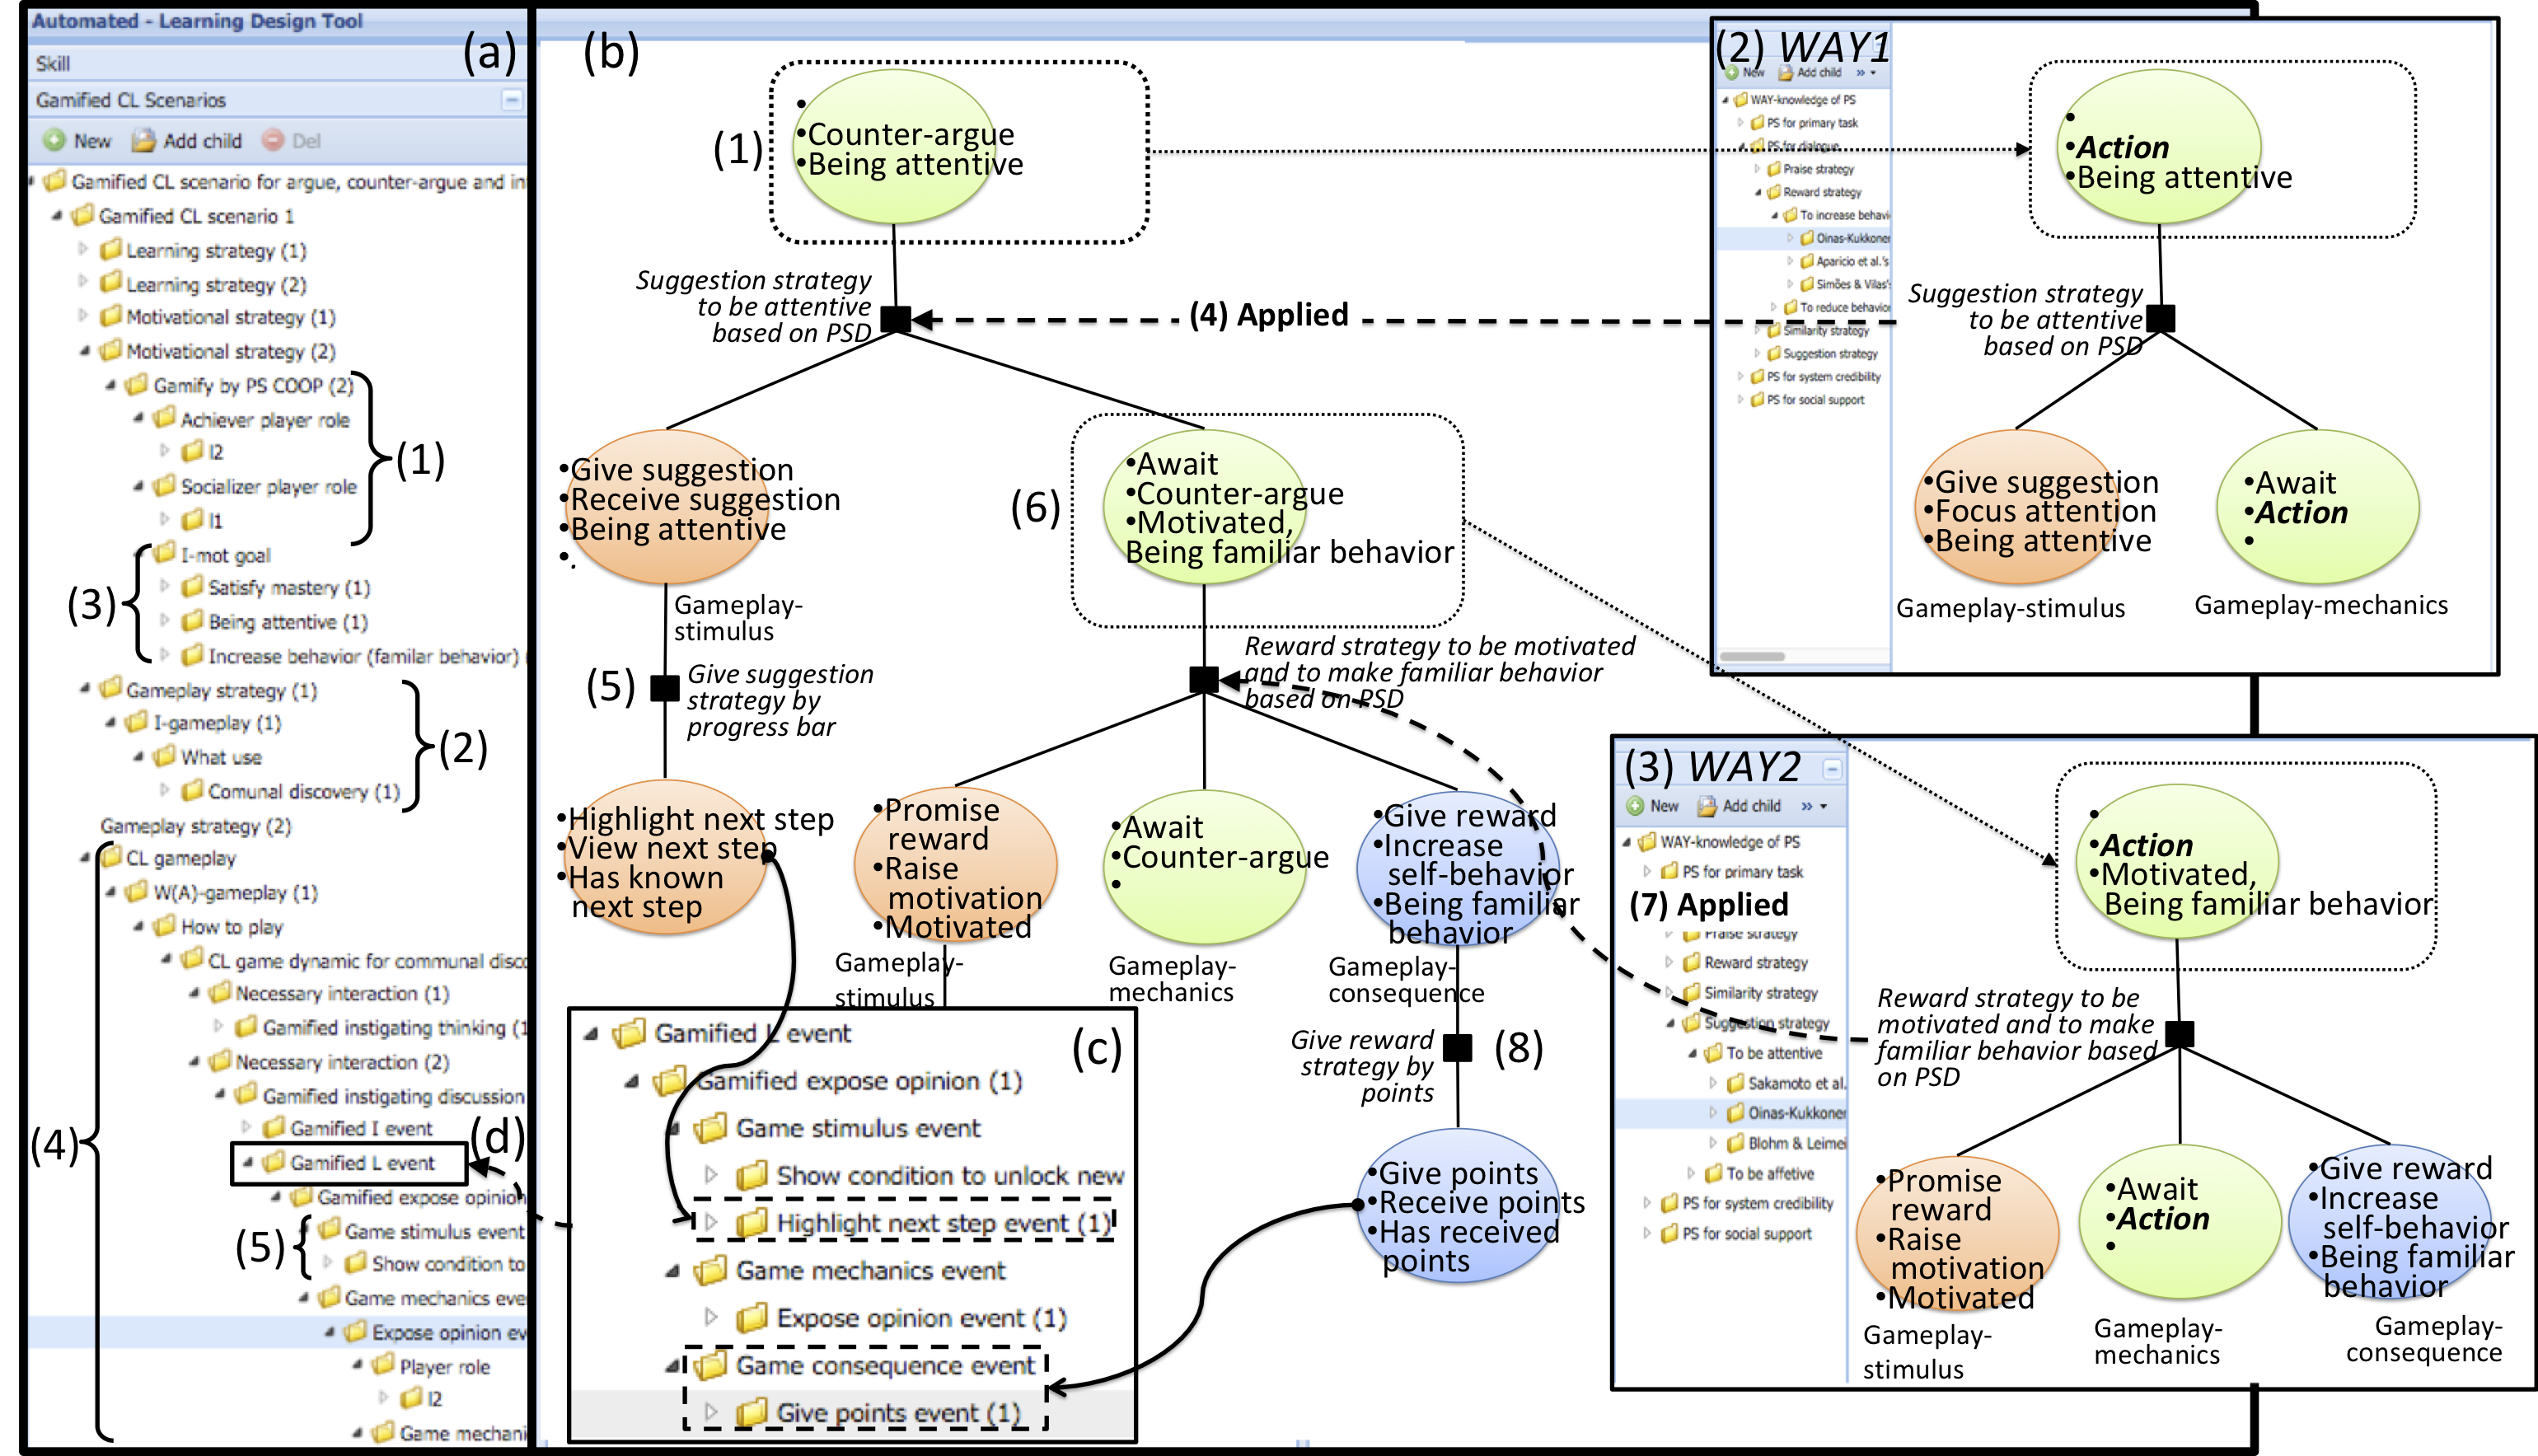
\includegraphics[width=1.5\textwidth]{images/chap-
%mechanisms-procedures/gamification-framework-editing-environment.png} % \fautor %\end{figure} %\end{landscape}


%To demonstrate the utility of our approach that consists of the concep-tualization of PSs presented in the previous
%section, we are developing an advanced authoring intelligent theory-aware system based on the refer-ence architecture
%shown in Fig. 4. Fig. 9 illustrates the manner in which this theory-aware system uses the WAY-knowledge base of PSs to
%gam-ify a CL scenario during the CL gameplay design. In this example, as we show in Fig. 9 (a), the CL scenario being
%gamified is a scenario based on the CSCL script for “argumentation, counter-argumentation and inte-gration” proposed by
%Stegmann et al. in [33]. After the selection of player roles and games elements for each student of CL scenario, as
%shown in Fig. 9 (a-1), the socializer role is assigned for the student l1 who has the role of arguer, while the
%achiever role is assigned for the student l2 who has the role of co-arguer. Fig. 9 (a-1) also shows that the
%motivational strategies for socializers and achievers are the “Gamifying by persuasive strategy COOP,” in both cases.
%Fig. 9 (a-2) shows that the selected game elements in gameplay strategy (I-gameplay strategy) for socializer and
%achiever are the communal discovery. Finally, the individual motivation goals (I-mot goal) for students l2 are “satisfy
%mastery,” “be attentive” and “increase behavior (familiar behavior)” as shown in Fig 9 (a-3).
  
%Fig. 9. Illustration of how to employ the WAY-knowledge base of Persuasive Strategies. The default “CL gameplay” for
%the scenario shown in Fig. 9 (a-4) is obtained by employing an ontological model that extends the ontological
%structures shown in Fig. 3. This model employs the information defined by Orji et al. in [29], and its detail of
%construction can be found in [3]. As result of the application of this model, each gamified instructional and learning
%event defines the game action “show condition to unlock new content” as game stimulus event that persuades the student
%l2 to do the actions of learning event as shown in Fig. 9 (a-5). Employing the WAY-knowledge base of PSs, we can
%personalize the gamified instructional and learning event for each student of a gamified CL scenario by adding new game
%stimulus and game consequences events, so that the Fig. 9 (b) shows how this personalization is done for the student l2
%over the learning event “expose opinion.” First, after the selection of the event that will be personalized, the macro-
%gameplay event is automatically filled by the information of selected event as shown in Fig. 9 (b-1). Based in the
%individual motivational goals “be attentive” and “increase behavior (familiar behavior)” of student l2, the system pro-
%poses the ways of decomposition WAY1 and WAY2, respectively shown in Fig. 9 (b-2) and Fig. 9 (b-3). The first way
%(WAY1) emerges from the PS “Oinas-Kukkonen & Harjumaa’s suggestion strategy to be attentive” because it allows to “be
%attentive” (I-mot goal). The second way (WAY2) emerges from the PS “Oinas-Kukkonen & Harjumaa’s reward strategy to
%increase behavior” because it allows to “increase behavior (familiar behavior).” In this example, the designer selects
%the first way (WAY1) decomposing the macro-gameplay (Fig. 9 (b-1)) into two micro-gameplay events with the game actions
%“give suggestion” and “awaiting action” as shown in Fig. 9 (b-4). The designer can decompose the game action “give
%suggestion” by employing different PSs. For this example, the designer selects the PS “Orji et al.’s suggest by
%progress bar” as shown in Fig. 9 (b-5). Next, the designer decomposes the gameplay me-chanics event shown in Fig. 9
%(b-6) into two micro-gameplay events with the game actions “awaiting action” and “give reward” as shown in Fig. 9
%(b-7). This decomposition emerges from the PS “Oinas-Kukkonen & Harjumaa’s reward strategy to increase behavior” (WAY2)
%shown in Fig. 9 (b-3). Finally, the game action “give reward” is decomposed into the game action “give points” by the
%application of PS “Orji et al.’s re-ward by points” shown in Fig. 9 (b-8). The process to personalize the gamified
%instructional and learning event shown in Fig. 9 (b) can be repeated for each student and over each instructional and
%learning event to define a better gamified CL scenario. At the end of this process, as shown in Fig. 9 (c), the system
%integrates the game events in a set of game stimulus and game consequence events. For this example, the game action
%“highlight next step” done by the “progress bar system” is integrated into a game stimulus event, and the game action
%“give points” done by the “point system” is integrated in a game consequence event. Finally, the last step is the
%addition of game stimulus and game consequence events into its respective gamified event as shown in Fig. 9 (d).




